
\begin{frame}
\frametitle{Admissibility gives low-rank}

\begin{figure}%[scale=0.8]
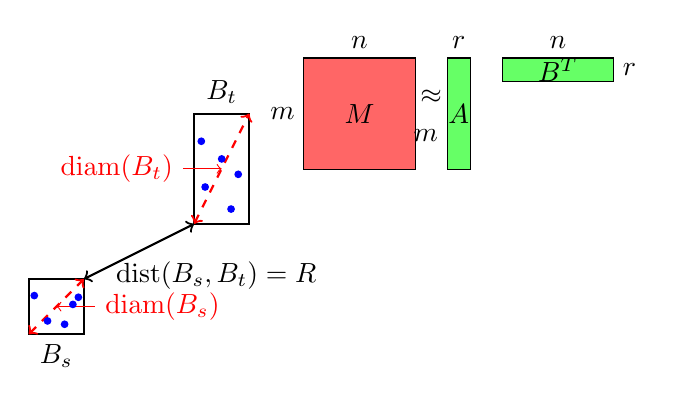
\begin{tikzpicture}[scale=0.7]
\draw[thick] (4,1) rectangle (5,2);
\draw[thick] (7,3) rectangle (8,5);
\draw[thick,<->,dashed,red] (4,1) -- (5,2);
\draw[thick,<->,dashed,red] (7,3) -- (8,5);
\draw[thick,red] (5.2,1.5) node[right]{$\mathrm{diam}(B_s)$};
\draw[thin,red,<-] (4.5,1.5)--(5.2,1.5);
\draw[thick,red] (6.8,4) node[left]{$\mathrm{diam}(B_t)$};
\draw[thin,red,->] (6.8,4)--(7.5,4);
\draw[thick,<->] (5,2) -- (7,3);
\draw[thick] (7.4,2.5) node[below]{$\mathrm{dist}(B_s,B_t)=R$};
\draw[thick] (4.5,1) node[below]{$B_s$};
\draw[thick] (7.5,5) node[above]{$B_t$};

\fill[blue] (4.1,1.7) circle[radius=2pt];
\fill[blue] (4.65,1.18) circle[radius=2pt];
\fill[blue] (4.8,1.54) circle[radius=2pt];
\fill[blue] (4.9,1.67) circle[radius=2pt];
\fill[blue] (4.34,1.24) circle[radius=2pt];

\fill[blue] (7.2, 3.67) circle[radius=2pt];
\fill[blue] (7.5, 4.18) circle[radius=2pt];
\fill[blue] (7.80, 3.90) circle[radius=2pt];
\fill[blue] (7.13, 4.50) circle[radius=2pt];
\fill[blue] (7.67, 3.27) circle[radius=2pt];


  \draw[thick=1] (9,4) rectangle (11,6);
  \fill[red!60!white] (9,4) rectangle (11,6);
  \node at (10.0,5.0) {$M$};
  \node[above] at (11.3,5.0) {$\approx$};
  \node[left] at (9.0,5.0) {$m$};
  \node[above] at (10.0,6.0) {$n$};



  \draw[thick] (11.6,4) rectangle (12.0,6.0);
  \fill[green!60!white](11.6,4) rectangle (12.0,6.0);
  \node at (11.8,5.0) {$A$};
  \node[left] at (11.6,4.6) {$m$};
  \node[above] at (11.8,6.0) {$r$};



  \draw[thick] (12.6,5.6) rectangle (14.6,6.0);
  \fill[green!60!white](12.6,5.6) rectangle (14.6,6.0);
  \node at (13.6,5.8) {$B^T$};
  \node[right] at (14.6,5.8) {$r$};
  \node[above] at (13.6,6.0) {$n$};

\end{tikzpicture}
\end{figure}

Usual condition:
\[
\min(\mathrm{diam}(B_t),\mathrm{diam}(B_s)) \leqslant \eta \, \mathrm{dist}(B_t,B_s) \qquad \text{(admissibility condition)}
\]

The separation condition $R=0$ gives the \textbf{HODLR}(\textbf{H}ierarchically \textbf{O}ff-\textbf{D}iagonal \textbf{L}ow-\textbf{R}ank) structure described by the 1D toy model.
\end{frame}

